\section{Pilot Results}
\label{sec:pilot-results}

This section reports controlled pilot results. They should be read as feasibility evidence for the proposed risk-calibrated selector, not as a claim of state-of-the-art KV cache compression. The experiments use small synthetic retrieval prompts and a small instruction-tuned model. Their role is to test whether the instrumentation works, whether risk tolerance behaves as a usable control knob, and whether a conservative \uckv{} operating point can match high-retention baselines while retaining fewer tokens.

\subsection{Metrics and evaluation protocol}

The pilot records two kinds of metrics. \emph{Replay metrics} force each compressed policy to follow the full-cache token path and measure the KL divergence and top-1 mismatch of next-token logits. These metrics isolate local distribution perturbation. \emph{Free-running metrics} let each compressed policy generate its own continuation and then check whether the expected answer string appears in that continuation. Free-running answer containment is closer to task behavior, but it remains a coarse metric on small prompt sets.

We use SmolLM2-135M-Instruct with the tokenizer chat template. Earlier raw-prompt runs gave poor full-cache retrieval accuracy and are treated only as diagnostics. This matters because cache compression comparisons are meaningful only after the full-cache prompt format is known to solve the task at a reasonable rate.

\subsection{Final SmolLM2 retrieval suite}

The final suite first runs a 144-prompt main sweep with seed 29. The fixed baselines are full cache and sink-plus-window retention with four protected sink tokens and recent windows $\{64,128,192,\allowbreak 256,320,384\}$. The \uckv{}-Budget sweep then reuses the fixed-window replay traces to evaluate risk tolerances from 0.30 to 0.50. The answer-containment metrics for the \uckv{} sweep are real free-running generations; the replay KL and top-1 mismatch metrics for those tolerance-sweep rows are fixed-candidate simulations from the source replay.

Table~\ref{tab:final-seed29} shows the main operating region. The best fixed-window baseline is sink+window 384, which matches full-cache answer containment at 0.9306 while retaining 283.93 tokens on average. \uckv{} at tolerance 0.36 also reaches 0.9306 answer containment, while retaining 259.21 tokens on average. Increasing the tolerance beyond 0.36 gives a sharp quality drop: tolerance 0.365 falls to 0.8889, and tolerance 0.40 falls to 0.7917. Thus the useful boundary is narrow but identifiable.

\begin{table}[t]
\centering
\small
\caption{Main SmolLM2-135M-Instruct retrieval sweep on seed 29, evaluation split. UCKV free-running answer containment is measured by real generation; UCKV replay metrics in this sweep are fixed-candidate simulations.}
\label{tab:final-seed29}
\begin{tabular}{lrrrr}
\toprule
Policy & Answer contain. & Avg kept & Avg KL & Fallback steps \\
\midrule
Full KV & 0.9306 & 287.60 & 0.0000 & 0 \\
Sink+window 256 & 0.7639 & 235.96 & 0.1300 & 0 \\
Sink+window 320 & 0.8472 & 267.14 & 0.0647 & 0 \\
Sink+window 384 & 0.9306 & 283.93 & 0.0006 & 0 \\
\uckv{} tol. 0.34 & 0.9306 & 274.13 & 0.0008 & 240 \\
\uckv{} tol. 0.35 & 0.9306 & 266.42 & 0.0009 & 181 \\
\uckv{} tol. 0.36 & 0.9306 & 259.21 & 0.0011 & 159 \\
\uckv{} tol. 0.365 & 0.8889 & 255.51 & 0.0013 & 153 \\
\uckv{} tol. 0.40 & 0.7917 & 237.65 & 0.0647 & 53 \\
\uckv{} tol. 0.50 & 0.6806 & 190.61 & 0.1389 & 20 \\
\bottomrule
\end{tabular}
\end{table}

\begin{figure}[t]
\centering
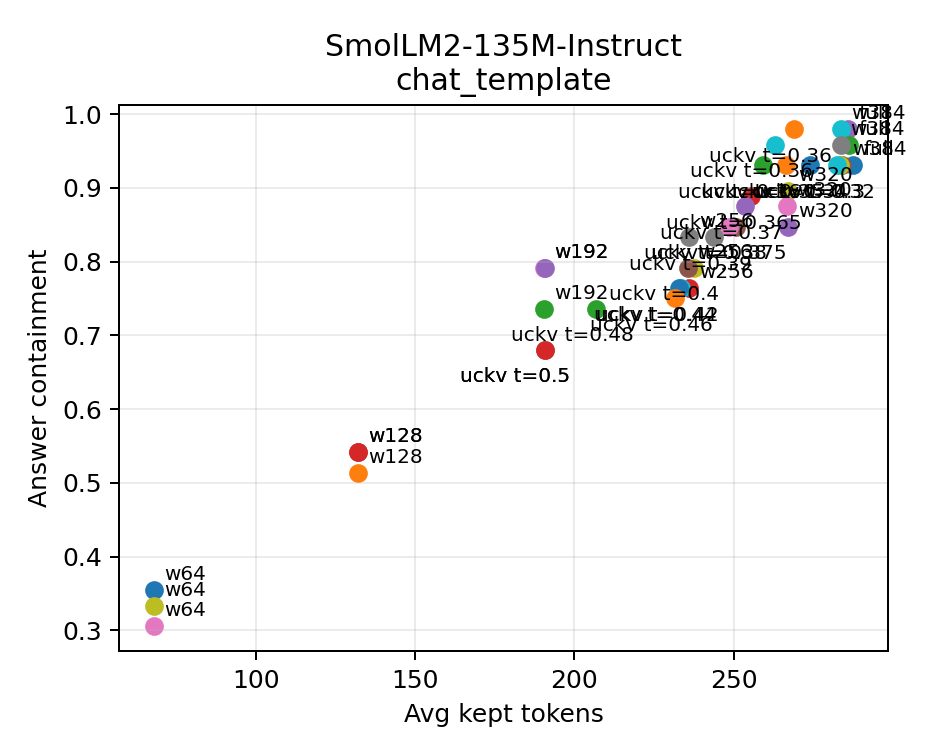
\includegraphics[width=\linewidth]{figures/retrieval-tradeoff.png}
\caption{Free-running retrieval tradeoff for the final SmolLM2 pilot. The selected operating point is \uckv{} tolerance 0.36: it matches the high-retention accuracy frontier on the main sweep while reducing retained tokens relative to full cache and sink+window 384.}
\label{fig:retrieval-tradeoff}
\end{figure}

\subsection{Confirmation seeds}

After selecting tolerance 0.36 from the seed-29 sweep, we run two confirmation seeds, 31 and 37, with 96 prompts each. These confirmation runs execute actual replay and actual free-running generations for all policies. Table~\ref{tab:final-confirm} reports the aggregate over the two confirmation seeds. \uckv{} matches the mean and minimum answer containment of both full-cache decoding and sink+window 384, while retaining fewer tokens on average.

\begin{table}[t]
\centering
\small
\caption{Confirmation seeds for SmolLM2-135M-Instruct, evaluation split. The selected \uckv{} tolerance is 0.36. Metrics are averaged across seed 31 and seed 37; all rows use actual replay and actual free-running generations.}
\label{tab:final-confirm}
\begin{tabular}{lrrrr}
\toprule
Policy & Seeds & Mean answer & Min answer & Avg kept \\
\midrule
Full KV & 2 & 0.9688 & 0.9583 & 286.07 \\
Sink+window 384 & 2 & 0.9688 & 0.9583 & 283.60 \\
\uckv{} tol. 0.36 & 2 & 0.9688 & 0.9583 & 266.10 \\
Sink+window 320 & 2 & 0.8854 & 0.8750 & 266.95 \\
Sink+window 256 & 2 & 0.8125 & 0.7917 & 235.79 \\
Sink+window 192 & 2 & 0.7917 & 0.7917 & 190.55 \\
Sink+window 128 & 2 & 0.5417 & 0.5417 & 132.00 \\
Sink+window 64 & 2 & 0.3438 & 0.3333 & 68.00 \\
\bottomrule
\end{tabular}
\end{table}

Relative to full cache, \uckv{} reduces retained tokens from 286.07 to 266.10, a 7.0\% reduction at the same answer-containment accuracy. Relative to the strongest fixed-window baseline, sink+window 384, it reduces retained tokens from 283.60 to 266.10, a 6.2\% reduction. These savings are modest, but they are achieved without reducing answer containment in the confirmation seeds.

\subsection{UCKV2 matched-budget gate}

The first \uckv{}-Budget pilots above identify useful instrumentation, but the resulting selector is conservative and does not directly compete with strong H2O-style heavy-hitter retention at a fixed cache budget. We therefore implemented a second-stage selector, denoted UCKV2 in the experiment code, that reuses the H2O attention-accumulation loop but gates attention updates by next-token uncertainty and adds prefill salience. This gate tests whether uncertainty can improve the heavy-hitter score itself, rather than only selecting among sink-window sizes.

The matched-budget gate compares H2O and UCKV2 at budgets $\{96,128,192,256\}$ on five independent SmolLM2 seeds, using 96 retrieval prompts per seed and the same chat-template, greedy decoding, and 24-token generation budget. Table~\ref{tab:uckv2-l1} reports evaluation-split answer containment averaged over seeds. The 256-budget point is the main signal: UCKV2 improves answer containment from 0.6708 to 0.8708 while retaining only 3.11 more tokens on average. The paired prompt comparison has 240 evaluation prompts; at budget 256, H2O is uniquely correct on 0 prompts and UCKV2 is uniquely correct on 48 prompts. A paired bootstrap gives a 95\% interval of $[0.1500,0.2542]$ for the answer-containment delta, and an exact McNemar test gives $p=7.11\times10^{-15}$.

\begin{table}[t]
\centering
\small
\caption{UCKV2 matched-budget gate on SmolLM2-135M-Instruct, evaluation split. Metrics are averaged over five seeds. ``Delta'' is UCKV2 minus H2O answer containment.}
\label{tab:uckv2-l1}
\begin{tabular}{rrrrrr}
\toprule
Budget & H2O answer & UCKV2 answer & Delta & H2O kept & UCKV2 kept \\
\midrule
96 & 0.4917 & 0.4667 & -0.0250 & 96.00 & 101.88 \\
128 & 0.4917 & 0.5167 & +0.0250 & 128.00 & 133.88 \\
192 & 0.5958 & 0.6042 & +0.0083 & 187.80 & 192.21 \\
256 & 0.6708 & 0.8708 & +0.2000 & 233.95 & 237.06 \\
\bottomrule
\end{tabular}
\end{table}

\begin{figure}[t]
\centering
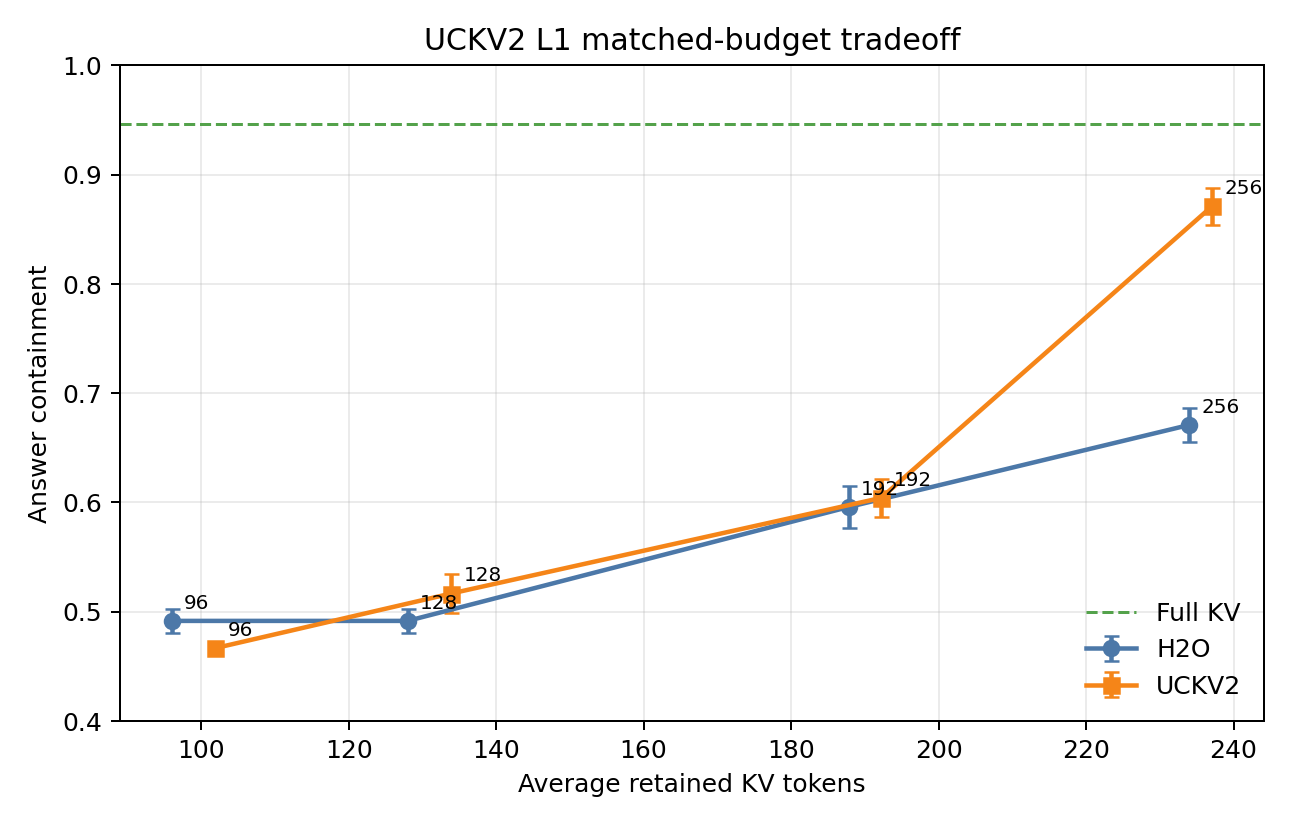
\includegraphics[width=0.86\linewidth]{figures/uckv2-l1-tradeoff.png}
\caption{UCKV2 matched-budget gate on SmolLM2-135M-Instruct. UCKV2 is not useful at the smallest budget, but it substantially improves the 256-token operating point relative to the H2O baseline.}
\label{fig:uckv2-l1-tradeoff}
\end{figure}

These local results are not a full benchmark claim. They are a gate for deciding whether the redesigned selector is worth a larger-model confirmation. The gate passes for budget 256, is weakly positive at 128 and 192, and fails at 96.

\subsection{Qwen2.5-7B confirmation of UCKV2}

We then ran the matched-budget confirmation on Qwen2.5-7B-Instruct on DGX Spark, using five independent seeds, 72 prompts per seed, the same controlled retrieval template, greedy decoding, and budgets $\{128,192,256\}$. This confirmation did not reproduce the SmolLM2 gain. Table~\ref{tab:uckv2-qwen25-7b} shows that H2O dominates the current UCKV2 selector at every tested budget: UCKV2 has lower answer containment, retains about 6.56 additional tokens, and incurs selector overhead during decoding.

\begin{table}[t]
\centering
\small
\caption{Qwen2.5-7B-Instruct DGX confirmation for UCKV2, evaluation split. Metrics are averaged over five seeds. ``Delta'' is UCKV2 minus H2O answer containment.}
\label{tab:uckv2-qwen25-7b}
\begin{tabular}{rrrrrr}
\toprule
Budget & H2O answer & UCKV2 answer & Delta & H2O kept & UCKV2 kept \\
\midrule
128 & 0.9444 & 0.6944 & -0.2500 & 128.00 & 134.56 \\
192 & 0.9333 & 0.7056 & -0.2278 & 192.00 & 198.56 \\
256 & 0.9278 & 0.7056 & -0.2222 & 256.00 & 262.56 \\
\bottomrule
\end{tabular}
\end{table}

\begin{figure}[t]
\centering
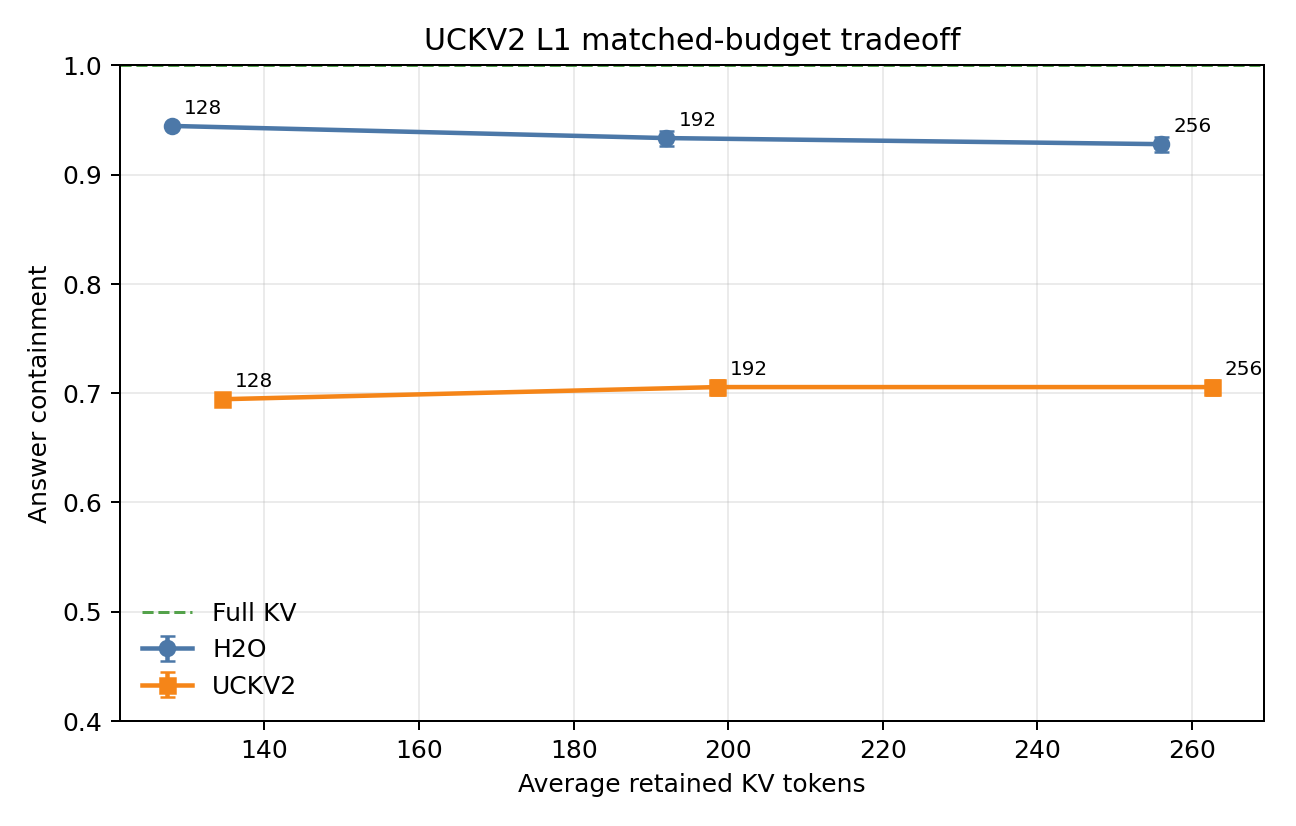
\includegraphics[width=0.86\linewidth]{figures/uckv2-qwen25-7b-tradeoff.png}
\caption{UCKV2 matched-budget confirmation on Qwen2.5-7B-Instruct. Unlike the SmolLM2 gate, the current UCKV2 selector is below H2O at all tested budgets on the 7B model.}
\label{fig:uckv2-qwen25-7b-tradeoff}
\end{figure}

The paired comparison contains 180 evaluation prompts. At budget 256, H2O is uniquely correct on 41 prompts, UCKV2 is uniquely correct on one prompt, the paired answer-containment delta is $-0.2222$, the bootstrap 95\% interval is $[-0.2833,-0.1611]$, and the exact McNemar test gives $p=1.96\times10^{-11}$. Thus the current UCKV2 selector fails the larger-model confirmation. We therefore treat the SmolLM2 result as a useful diagnostic signal, not as evidence that the current selector improves a 7B quality-memory frontier.

\subsection{Risk-tolerance boundary and failure modes}

The final sweep shows that tolerance is a real quality-efficiency control. From tolerance 0.34 to 0.36, answer containment remains at 0.9306 while average retained tokens fall from 274.13 to 259.21. At tolerance 0.365, answer containment drops to 0.8889, despite only a small additional token reduction. Larger tolerances continue to reduce retained tokens but degrade retrieval quality.

The position breakdown explains the cliff. At tolerance 0.36 on the seed-29 sweep, answer containment is 1.0000 for early-position answers, 0.8750 for middle answers, and 0.9167 for late answers. At tolerance 0.365, early-position containment falls to 0.8750 while middle and late positions remain unchanged. At tolerance 0.40, early-position containment falls to 0.5833. Thus the first visible failures come from evidence placement rather than from a uniform degradation across all prompts.

The context-length breakdown gives a complementary view. At tolerance 0.36, the seed-29 sweep retains high containment across context lengths: 0.8889 at 64 words, 0.9444 at 128 words, 1.0000 at 192 words, and 0.8889 at 256 words. For longer prompts, \uckv{} often falls back to the largest candidate window, which preserves quality but limits memory savings. This explains why the selected point is conservative.

\subsection{Pilot takeaways}

The pilot supports five modest conclusions. First, the replay/free-run pipeline can measure both local distribution perturbation and task-level degradation. Second, calibrated risk tolerance behaves as a usable memory-quality knob, with a clear boundary around 0.36 in the final SmolLM2 suite. Third, the selected \uckv{} point matches full cache and the strongest fixed-window baseline on the confirmation seeds while reducing retained tokens by 6--7\%. Fourth, uncertainty-gated heavy-hitter scoring can produce a strong local gain on SmolLM2, but the same selector fails on Qwen2.5-7B and is therefore not yet a validated scalable method. Fifth, the current implementation does not yet demonstrate broad benchmark or production serving speedups; the experiments measure retained-token counts, free-running answer containment, replay perturbation, and selector overhead on controlled runs.

The result is therefore useful but not yet positive enough for a main benchmark claim. It shows that uncertainty-calibrated cache control can be instrumented, stress-tested, and falsified under matched-budget conditions. The next method iteration should explain why the SmolLM2 gate does not transfer to Qwen2.5-7B, then retest only after a local matched-budget gate and a larger-model confirmation both pass.
